\pdfminorversion=4
\documentclass[]{article}

%%%%%%%%%%%%%%%%%%%
% Packages/Macros %
%%%%%%%%%%%%%%%%%%%
\usepackage{amssymb,latexsym,amsmath}     % Standard packages
\usepackage{graphicx}
\graphicspath{ {./images/} }
\usepackage{amsmath,amssymb}


%%%%%%%%%%%
% Margins %
%%%%%%%%%%%
\addtolength{\textwidth}{1.0in}
\addtolength{\textheight}{1.00in}
\addtolength{\evensidemargin}{-0.75in}
\addtolength{\oddsidemargin}{-0.75in}
\addtolength{\topmargin}{-.50in}


%%%%%%%%%%%%%%%%%%%%%%%%%%%%%%
% Theorem/Proof Environments %
%%%%%%%%%%%%%%%%%%%%%%%%%%%%%%
\newtheorem{theorem}{Theorem}
\newenvironment{proof}{\noindent{\bf Proof:}}{$\hfill \Box$ \vspace{10pt}}


%%%%%%%%%%%%
% Document %
%%%%%%%%%%%%
\begin{document}

\title{HW5}
\author{Amitesh Badkul}
\maketitle

\begin{abstract}
This document contains my attempt at the homework 5 problems of the course
Learning From Data ({\bf CS156}) as taught by Professor {\em Yaser Abu-Mostafa, Caltech}.
\end{abstract}


%%%%%%%%%%%%%%%
\begin{enumerate}
\item[$\bullet$] {\bf Overfitting and Deterministic Noise}
        \subitem {\small 1.[b]}
\includegraphics[scale=0.3]{noise}
\end{enumerate}

\item[$\bullet$] {\bf Regularization with Weight Decay}
    \begin{enumerate}
        \subitem {\small 2.[b], the in-sample error comes close to $0.08$ whereas the out-of-sample error turns out be $0.528$}
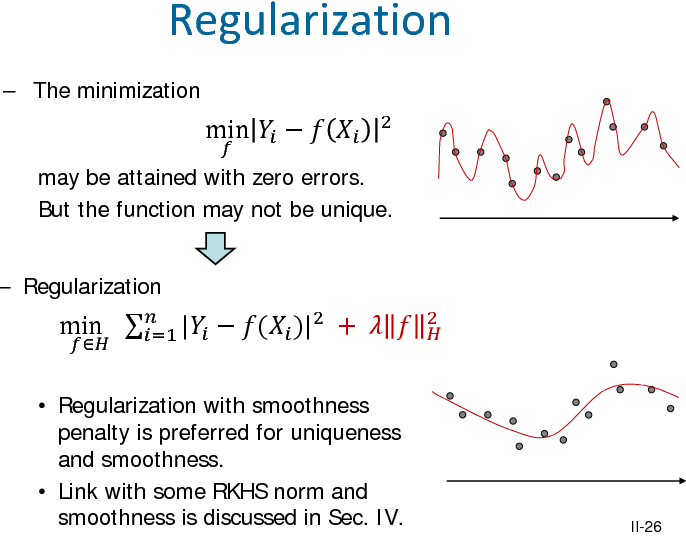
\includegraphics[scale=0.5]{reg}
        \subitem {\small 3.[a], values come out to be $0.007457366217152011 0.2787994598418299}
    \end{enumerate}



\item[$\bullet$] {\bf Regularization for Polynomials}
    \begin{enumerate}
        \subitem {\small 4.[e]}
        \subitem {\small 5.[d], by using different values of k in the regualrizer it can be obtained }
        \subitem {\small 6.[b], at $k = -1, 0.06$ value of out-sample error is acheived}
        \subitem {\small 7.[c], the first Hypothesis will give $\mathcal{H}2$ and second one will give $\mathcal{H}3$ and hence intersection of both will be $\mathcal{H}2$}
    \end{enumerate}

\item[$\bullet$] {\bf Neural Networks}
    \begin{enumerate}
        \subitem {\small 8.[d]}
        \subitem {\small 9.[a]}
    \end{enumerate}

\item[$\bullet$] {\bf }
    \begin{enumerate}
        \subitem {\small 10.[e]}
    \end{enumerate}

\end{enumerate}



\end{document}
